\section{Systemübersicht}
Folgend wird eine grobe Übersicht über das Lokkit System geschaffen. Komponenten werden benannt und deren Funktionalität grob erklärt. Für Implementationsspezifische Einzelheiten, vgl. \ref{sec:Komponenten}.

\subsection{Systemkontext}
Das Lokkit System wurde Komponentenweise entworfen und kann dementsprechend auch so installiert werden. Im Systemkontext wird jedoch der Einfachheit halber das System als Einheit dargestellt, mit der interagiert werden kann.
\begin{figure}
\centering
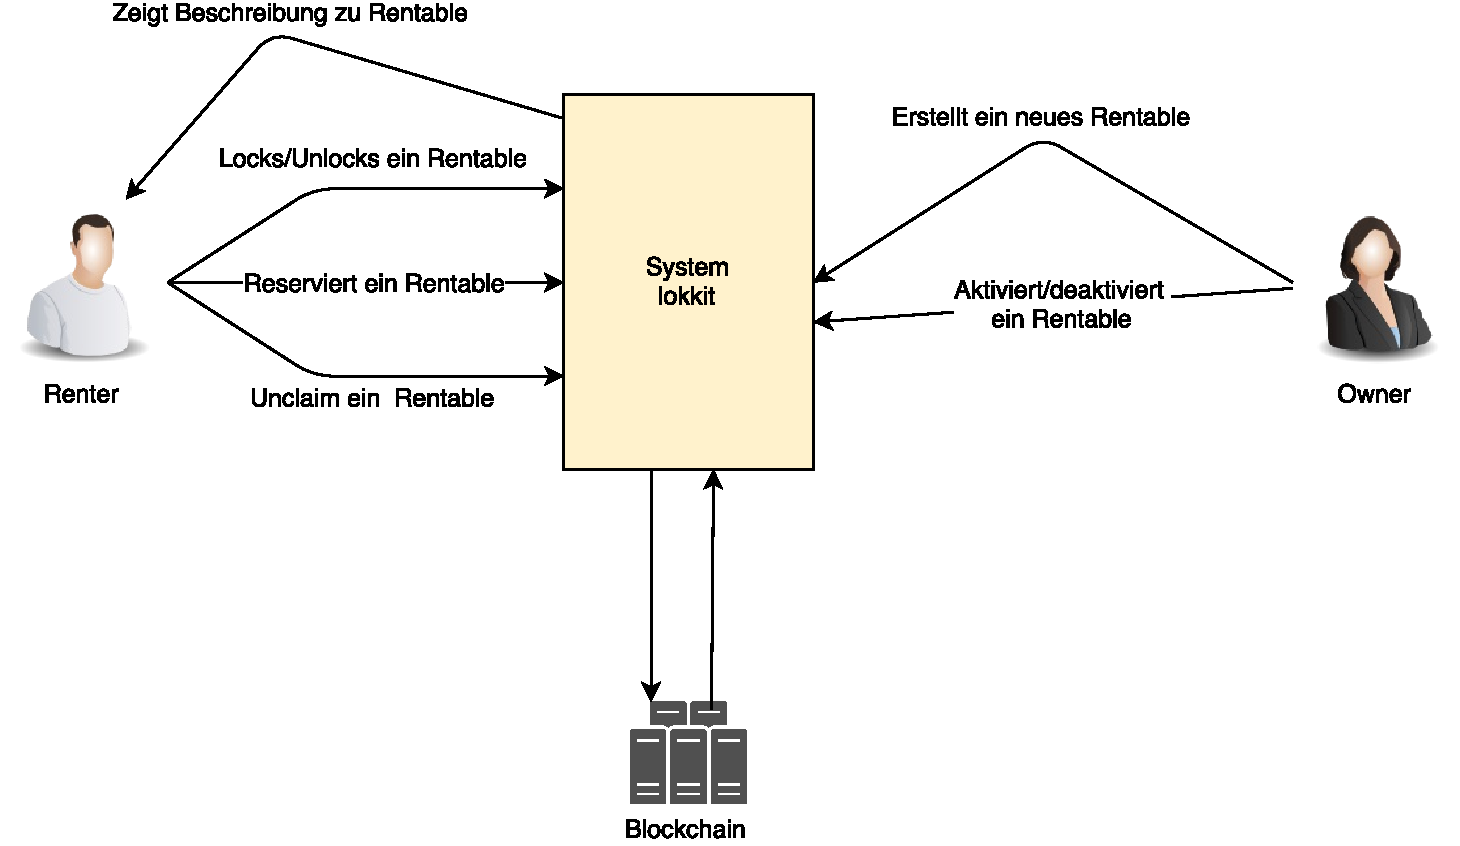
\includegraphics[width=.95\textwidth]{Kontext_Diagram}
\caption{Kontextdiagramm}
\label{fig:Kontextdiagramm}
\end{figure}

\subsection{Systemübersicht IoT}
\label{subsec:Setup_IoT}
Folgend wird das Setup der im Demonstrator zur Verfügung stehender Hardware aufgezeigt.
Übersicht: Raspis, Schliessfächer etc...
\begin{figure}
\centering
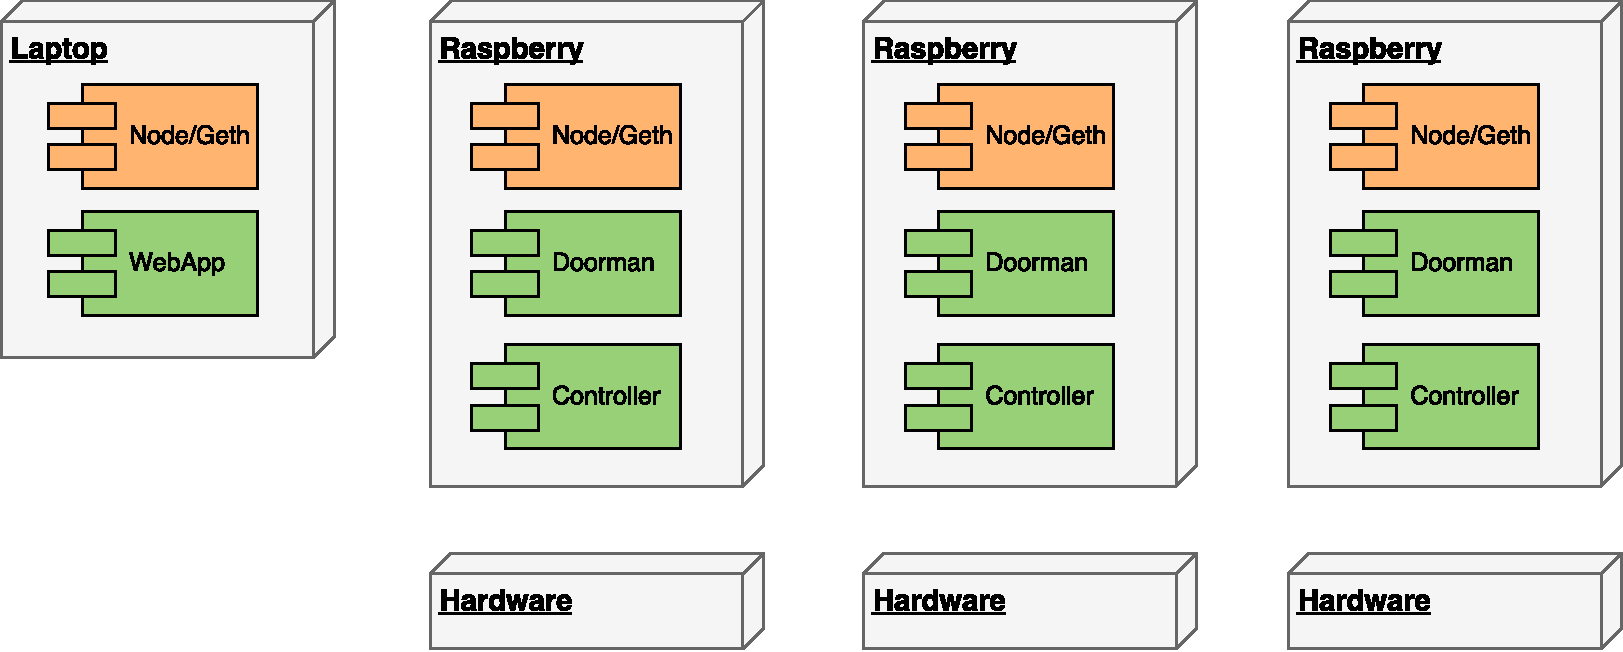
\includegraphics[width=.95\textwidth]{Aufbau_Komponenten}
\caption{Verteilung der Komponenten auf den IoT Geräten}
\label{fig:Aufbau Komponenten}
\end{figure}

\begin{figure}
\centering
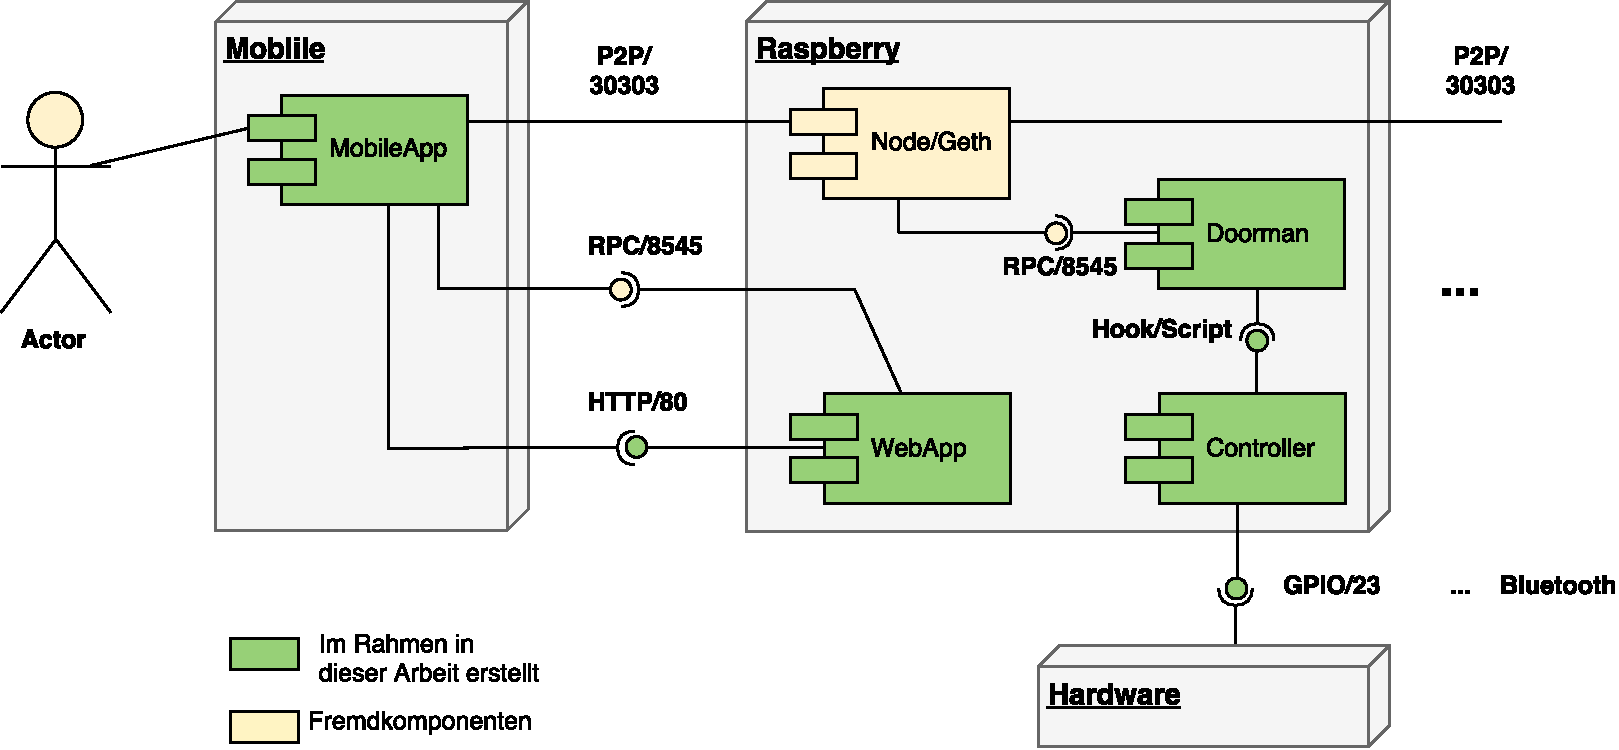
\includegraphics[width=.95\textwidth]{Aufbau_Komponenten_Interface}
\caption{Komponenten und Schnittstellen}
\label{fig:Komponenten und Schnittstellen}
\end{figure}



